%!TEX root =../../../course-notes.tex
% ^ leave for LaTeXTools build functionality
\begin{applicationActivities}

%30 minutes
\begin{observation}
There are two very simple kinds of separable ODEs.
\vfill
Equations of the form \(y'=f(x)\) can be solved immediately by integrating and produce explicit solutions.
\vfill
Equations of the form \(y'=f(y)\) are often impossible or difficult to solve explicitly.  They are called \term{autonomous} equations.
\end{observation}

\begin{activity}{10}
Consider the autonomous equation \[y'=y^2.\]
\vfill
\begin{subactivity}
Draw a slope field
\end{subactivity}
\begin{subactivity}
Suppose a solution goes through the point \(y(10)=50 \).  What can you say about \(y(11)\)?
\vfill
\begin{enumerate}[(a)]
\item \(y(10)<y(11)\)
\item \(y(10)=y(11)\)
\item \(y(10)>y(11)\)
\end{enumerate}
\end{subactivity}
\end{activity}

\begin{observation}
Since the slopes do not change when moving horizontally (i.e. in the \(x\) direction), we often collapse the slope field onto the \(y\)-axis.

\begin{multicols}{2}
\begin{center}
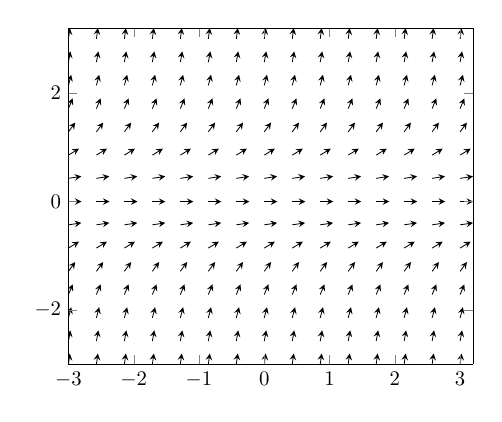
\begin{tikzpicture}[scale = 0.75]
    \begin{axis}[
        %title={\(y' = y^2 \)},
        domain=-3:3,
        view={0}{90},
        axis background/.style={fill=white},
    ]
        \addplot3[black,
            quiver={
             u={1/(sqrt(1 + (y^2)^2))},
             v={(y^2 )/(sqrt(1 + (y^2)^2))},
             scale arrows=0.2,
            },
            -stealth,samples=15]
                {exp(-x) - 1/2*sin(x) - 1/2*cos(x)};
    \end{axis}
\end{tikzpicture}
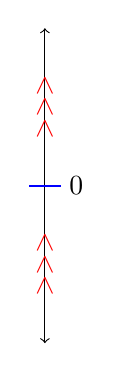
\begin{tikzpicture}
%\node at (-2.5,0) {\(y'\)};
\draw[<->] (0,-2) -- (0,2);
\draw[thick,blue] (-0.2,0) -- (0.2,0);
\node at (0.4,0) {\(0\)};
\node[red,rotate=90] at (0,-1) {\(>>>\)};
\node[red,rotate=90] at (0,1) {\(>>>\)};
\end{tikzpicture}

\end{center}
\end{multicols}

This is called a \term{phase line}.
\end{observation}

\begin{activity}{10}
Consider the autonomous equation \[y'=y^2(y-2).\]

\begin{subactivity}
Draw a number line for \(y'\), indicating where it is positive or negative.
\end{subactivity}
\begin{subactivity}
What can you say about the long term behavior of a solution passing through \(y(4)=1\)?
\end{subactivity}
\begin{subactivity}
What can you say about the long term behavior of a solution passing through \(y(2)=0.001\)?
\end{subactivity}
\begin{subactivity}
What can you say about the long term behavior of a solution passing through \(y(2)=-0.001\)?
\end{subactivity}
\end{activity}

\end{applicationActivities}
